% Long document, font size 12, two sides paper
\documentclass{report}

\linespread{1.5}
\setlength{\parskip}{1em}
\setlength{\parindent}{0em}

% Encoding format
\usepackage[utf8]{inputenc}

% Titles settings
\usepackage{titlesec}
\titleformat{\chapter}{\huge\bfseries}{\thechapter}{1ex}{}
\titlespacing{\chapter}{0pt}{-30pt}{20pt}

% Graphics import
% Specify image folder
\usepackage{graphicx}
\graphicspath{{img/}}

% Graphics generation
\usepackage{tikz}
\usetikzlibrary{positioning}

% Special functions
% Lagrange symbol
\usepackage{amsmath}
\usepackage{amssymb}

% Page sizes, margins, adjust for binding
\usepackage[a4paper,
            width=150mm,
            top=25mm,
            bottom=25mm,
            bindingoffset=6mm]{geometry}

% Header manipulation
% Title in header right odd - left even
% Page number in left odd - right even
% Chapter number and name in right odd
% Section number and name in left even
% Line rulers of 2pt up and 1pt down
\usepackage{fancyhdr}
\pagestyle{fancy}
\fancyhead{}
\fancyhead[RO, LE]{Zumobot case study}
\fancyfoot{}
\fancyfoot[LO, RE]{\thepage}
\fancyfoot[RO]{\leftmark}
\fancyfoot[LE]{\rightmark}
\renewcommand{\headrulewidth}{2pt}
\renewcommand{\footrulewidth}{1pt}

% Color definitions
\usepackage{color}
\definecolor{mypink}{rgb}{0.8,0.3,0.8}
\definecolor{mygreen}{rgb}{0,0.5,0}
\definecolor{myblue}{rgb}{0,0,0.5}
\definecolor{mygray}{rgb}{0.6,0.6,0.6}

% Formated code insertion package
% Defines language, tab, size, numbering, coloring, ...
\usepackage{listings}
\renewcommand{\lstlistingname}{Code snippet} % Change of Word for caption
\renewcommand{\lstlistlistingname}{List of \lstlistingname s}
\lstset{language        = Matlab,
        tabsize         = 2,
        basicstyle      = \scriptsize\ttfamily,
        numbers         = left,
        keywordstyle    = \color{myblue},
        morekeywords    = {},
        stringstyle     = \color{mypink},
        morestring      = [b]",
        identifierstyle = \color{black},
        numberstyle     = \color{mygray},
        emph            = [1]{},
        emphstyle       = [1]{\color{mypink}},
        commentstyle    = \color{mygreen},
        inputpath       = ../
}

% References management
\usepackage[backend=bibtex,
            bibstyle=ieee,
            citestyle=alphabetic]{biblatex}
\bibliography{report}

% Start of the document
\begin{document}

% Inserts title page from external file
% Start of the title page
\begin{titlepage}
  % Centered environment
  \begin{center}
    % Vertical space from top
    \vspace*{1cm}

    % Title text, bold, size
    \Huge
    \textbf{Zumobot case study}

    % Vertical space
    \vspace{0.5cm}

    % Subtitle text, size
    \LARGE
    {Control Theory Module}

    % Vertical space
    \vspace{3.5cm}

    % Authors, bold
    \textbf{Javier Reyes\\
            Hari Kumar Venkatesh}

    % Space until next element
    \vfill

    % Subtext
    {Homework assignment}

    % Vertical space
    \vspace{2cm}

    % Inserts logo, 30% width
    
\includegraphics[width=0.3\textwidth]{fh-logo.png}

    % Vertical space
    \vspace{1cm}

    % University text, size
    \Large
    {Master Embedded Systems for Mechatronics\\
    Dortmund University of Applied Sciences and Arts\\
    Germany}

    % Vertical space
    \vspace{0.5cm}

    % Date, size
    \large
    {\today}

  \end{center}
\end{titlepage}


% Insert table of contents
\tableofcontents

% Insert a list of figures
\listoffigures

% Inserts introduction from external file
\chapter*{Introduction}
% Start of Introduction chapter
One of the most used study cases in Control Theory is the Inverted Pendulum analysis, as it presents an unstable open-loop characteristic but is also possible to stabilize it on a closed-loop configuration.

Here we present the analysis of the Zumobot 32U4, a small robot available in the market. The Zumo 32U4 robot is a complete, versatile robot controlled by an Arduino-compatible ATmega32U4 microcontroller. The Zumo 32U4 robot can be programmed from a computer using any operating system that supports the Arduino environment.

TODO: Complete


% Inserts chapter from external file
\chapter{System Analysis}
% Start of Chapter 1 - System Analysis
An inverted pendulum can be represented as a rigid body pendulum connected to a cart moving on a horizontal axis. Controlling the stability of the Zumobot can be compared to balancing the inverted pendulum on the moving cart.

\begin{figure}[h]
	\centering
	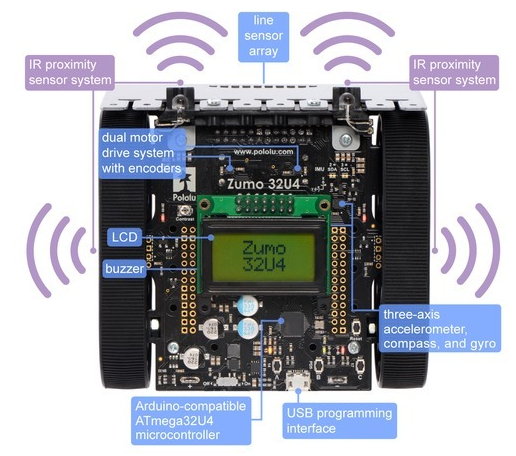
\includegraphics[width=0.5\textwidth]{zumo-superior.png}
	\caption{Superior view of the zumo robot.}
	\label{fig:sup-zumo}
\end{figure}

The figure \ref{fig:sup-zumo} shows the robot that will be modeled as a Wheeled Inverted Pendulum.

\begin{table}[h]
	\centering
	\caption{Basic table.}
	\label{tab:tab1}
	\begin{tabular}{ccc}
		\toprule
		header A & header B & header C\\
		\midrule
		a & b & c\\
		c & d & e\\
		f & g & h\\
		\bottomrule
	\end{tabular}
\end{table}

Text of the section\footnote{\label{fn1}This is a footnote}.

Text of the section after the footnote \ref{fn1}.

TODO: Complete.


% Inserts chapter from external file
\chapter{Mathematical Development}
% Start of Chapter 2 - Mathematical development

Through the numerous literature it is possible to find several approaches to obtain a model for the Inverted Pendulum elements. For this work the focus is mostly on the dynamic behavior of the robot, as it is the one that influences the most the response of the system. To completely model the dynamic behavior of the robot, we need to consider the equations that govern the movement as a rigid body.

\section{First approach: Forces analysis}

The first approach considered here is described in \cite{SUL03}. The methodology uses traditional dynamic physics to obtain the equations of motion. The final equation is then linearized and transformed into complex frequency domain.

\subsection{Dynamic behavior}

The equations of motion are obtained from the sum of forces in the cart for the horizontal direction (see figure \ref{fig:carforces}).

\begin{figure}[h]
	\centering
	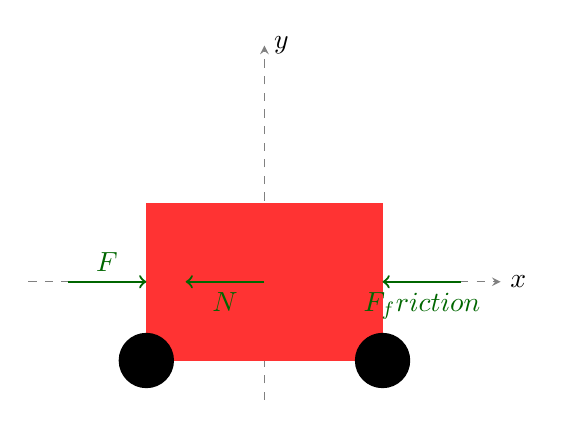
\begin{tikzpicture}
		[force/.style={->,thick,green!40!black}]
		% draw the two coordinate axis
		\draw [dashed,>=stealth,->, draw=gray] (-3,0) -- (3,0) node[anchor=west]{$x$};
		\draw [dashed,>=stealth,->, draw=gray] (0,-1.5) -- (0,3) node[anchor=west]{$y$};

		% draw the red mass with two wheels
		\fill[red!80!white] (-1.5,-1) rectangle (1.5,1);
		\fill (-1.5,-1) circle [radius=10pt];
		\fill (1.5,-1) circle [radius=10pt];

		%draw the forces
		\draw [force] (-2.5,0) -- node[green!40!black, auto]{$F$} (-1.5,0);
		\draw [force] (2.5,0) -- node[green!40!black, auto]{$F_friction$} (1.5,0);
		\draw [force] (0,0) -- node[green!40!black, auto]{$N$} (-1,0);
	\end{tikzpicture}
	\caption{Cart forces}\label{fig:carforces}
\end{figure}

\begin{equation} \label{sfch}
	F-b\cdot \dot{x}-N=M\cdot \ddot{x}
\end{equation}

Now considering the pendulum itself, the force applied in the horizontal direction due to the momentum of the pendulum is determined as:

\begin{figure}[h]
	\centering
	\begin{tikzpicture}
		[force/.style={->,thick,green!40!black}]
		% draw the two coordinate axis
		\draw [dashed,>=stealth,->, draw=gray] (-3,0) -- (3,0) node[anchor=west]{$x$};
		\draw [dashed,>=stealth,->, draw=gray] (0,-1.5) -- (0,3) node[anchor=west]{$y$};

		% draw the pendulum
		\node [circle,draw,blue,inner sep=0pt,minimum size=20pt] (pen) at (70:3) {};
		\draw[blue] (0,0) -- (pen);

		%draw the forces
		\draw [force] (70:1.5) -- node[green!40!black, auto]{$mg$} +(-90:1);
		\draw [force] (-1,0) -- node[green!40!black, auto]{$N$} (0,0);
		\draw [force] (70:1.5) -- node[green!40!black, auto]{$I\ddot{\theta}$} +(160:1);
		\draw [force] (70:3) -- node[green!40!black, auto]{$I\dot{\theta}^2$} +(70:1);
	\end{tikzpicture}
	\caption{Pendulum forces}\label{fig:penforces}
\end{figure}

\begin{equation} \label{dhfp}
	\tau=r\cdot F=I\cdot \ddot{\theta}
\end{equation}

Given the fact that the moment of inertia of a pendulum of mass $m$ is defined as $I=m\cdot L^2$, the previous equation can be rewritten as:

\begin{equation} \label{dhfp2}
	F=\frac{I\cdot \ddot{\theta}}{r}=\frac{m\cdot l^2\cdot \ddot{\theta}}{l}=m\cdot l\cdot \ddot{\theta}
\end{equation}

Obtaining the component of the force defined in \ref{dhfp2} in the horizontal direction:

\begin{equation} \label{sfph}
	F=m\cdot l\cdot \ddot{\theta}\cdot \cos{\theta}
\end{equation}

Now, the component of the centripetal force acting on the pendulum is similar to the one in \ref{dhfp2}, but the horizontal component of this force is:

\begin{equation} \label{cfph}
	F=m\cdot l\cdot \dot{\theta}^2\cdot \sin{\theta}
\end{equation}

Summing the defined forces present in the horizontal direction of the pendulum in \ref{sfph} and \ref{cfph}, we obtain the following expression:

\begin{equation} \label{nfp}
	N=m\cdot \ddot{x}+m\cdot l\cdot \ddot{\theta}\cdot \cos{\theta}-m\cdot l\cdot \dot{\theta}^2\cdot \sin{\theta}
\end{equation}

Now we can substitute \ref{nfp} into \ref{sfch}, we obtain the first equation of motion:

\begin{equation} \label{fem}
	F=(M+m)\ddot{x}+b\cdot \dot{x}+m\cdot l\cdot \ddot{\theta}\cdot \cos{\theta}-m\cdot l\cdot \dot{\theta}^2\cdot \sin{\theta}
\end{equation}

To get the second equation of motion, we sum the forces perpendicular to the pendulum. The vertical components of this forces are considered here to get:

\begin{equation} \label{sfppv}
	P\cdot \sin{\theta}+N\cdot \cos{\theta}-m\cdot g\cdot \sin{\theta}=m\cdot l\cdot \ddot{\theta}+m\cdot \ddot{x}\cdot \cos{\theta}
\end{equation}

To get rid of the $P$ and $N$ terms, sum the moments around the center of gravity of the pendulum:

\begin{equation} \label{smcg}
	-P\cdot l\cdot \sin{\theta}-N\cdot l\cdot \cos{\theta}=I\cdot \ddot{\theta}
\end{equation}

Summing up the equations \ref{sfppv} and \ref{smcg}, we obtain the second equation of movement:

\begin{equation} \label{sem}
	(I+m\cdot l^2)\ddot{\theta}+m\cdot g\cdot l\cdot \sin{\theta}=-m\cdot l\cdot \ddot{x}\cdot \cos{\theta}
\end{equation}

The obtained equations are non-linear, so they are linearized around the operating point, defined as the top vertical position or $\pi rad$ from the stable equilibrium position. We need also to define a small angle deviation from the top vertical position, so that $\theta=\pi+\phi$.

Under this circumstances, we can deduce that $\cos{\theta}\approx -1$, $\sin{\theta}\approx -\phi$, and $\dot{\theta}^2\approx 0$. Applying this relations into our movement equations, we obtain:

\begin{equation} \label{feml}
	F=(M+m)\ddot{x}+b\cdot \dot{x}-m\cdot l\cdot \ddot{\phi}
\end{equation}

\begin{equation} \label{seml}
	(I+m\cdot l^2)\ddot{\phi}-m\cdot g\cdot l\cdot \phi=m\cdot l\cdot \ddot{x}
\end{equation}

To obtain the transfer function of the linearized system of equations analytically, we perform the Laplace transform of the system equations:

\begin{equation} \label{fems}
	F(s)=(M+m)s^2\cdot X(s)+b\cdot s\cdot X(s)-m\cdot l\cdot s^2\cdot \Phi(s)
\end{equation}

\begin{equation} \label{sems}
	(I+m\cdot l^2)s^2\cdot \Phi(s)-m\cdot g\cdot l\cdot \Phi(s)=m\cdot l\cdot s^2\cdot X(s)
\end{equation}

To unify the equations, we solve \ref{fems} for $X(s)$ and then replace it into \ref{sems}, obtaining:

\begin{equation} \label{ecms}
	\frac{\Phi(s)}{F(s)}=\frac{m\cdot l\cdot s}{q\cdot s^3+b(l+m\cdot l^2)s^2-m\cdot g\cdot l(M+m)s-b\cdot m\cdot g\cdot l}
\end{equation}

Where:

\begin{equation} \label{dq}
	q=(M+m)(l+m\cdot l^2)-(m\cdot l)^2
\end{equation}

Assuming a coefficient of friction as zero, we can represent the equation as:

\begin{equation} \label{efms}
	\frac{\Phi(s)}{F(s)}=\frac{K_p}{\frac{s^2}{A_p^2}-1}
\end{equation}

With:

\begin{equation} \label{dka}
	K_p=\frac{1}{(M+m)g} ; A_p=\pm \sqrt{\frac{(M+m)m\cdot g\cdot l}{(M+m)(l+m\cdot l^2)-(m\cdot l)^2}}
\end{equation}

Considering that the Zumobot is a unique mass element, where a differentiation of cart and pendulum masses is not feasible, an adjustment of the equation \ref{dka} is made, so that the mass considered is the total mass of the robot. This is possible as the actuator system should face the entire mass of the robot, and the pendular mass is also corresponding to the complete body.

\begin{equation} \label{dka2}
	K_p=\frac{1}{mg} ; A_p=\pm \sqrt{\frac{m^2\cdot g\cdot l}{m(l+m\cdot l^2)-(m\cdot l)^2}}
\end{equation}

\subsection{Actuator system}

The actuation mechanism consist on a DC motor that drives a belt system around two wheels. The overall transfer function of the actuation mechanism will depend upon the motor and the belt system.

The torque to be delivered by the motor is:

\begin{equation} \label{t}
	T_L=(M+m)r^2\dot{\omega}
\end{equation}

The relation between Torque and Force can be expressed as:

\begin{equation} \label{dtf}
	T_L\propto r^2 ; F\propto r
\end{equation}

The motor dynamics can be represented with the well known transfer function, as in \cite{SUL03} \cite{ZAC17}:

\begin{equation} \label{md}
	\omega(s)=K_m\frac{V(s)}{\tau s+1}
\end{equation}

Where $\tau$ is the time constant and depends on the load, and $K_m$ is the steady-state gain of the motor.

\begin{equation} \label{mtf}
	\frac{T(s)}{E(s)}=K_m\frac{(M+m)r\cdot s}{\tau s+1}
\end{equation}

\subsection{Simulation}

The obtained model is analyzed with computational tools (MATLAB), to validate its behavior and calculate an appropriate controller. As shown in figure \ref{fig:zpopenA}, the system has a pole in the right part of the complex plane, fitting in the definition of an unstable system.

\begin{figure}[h]
	\centering
	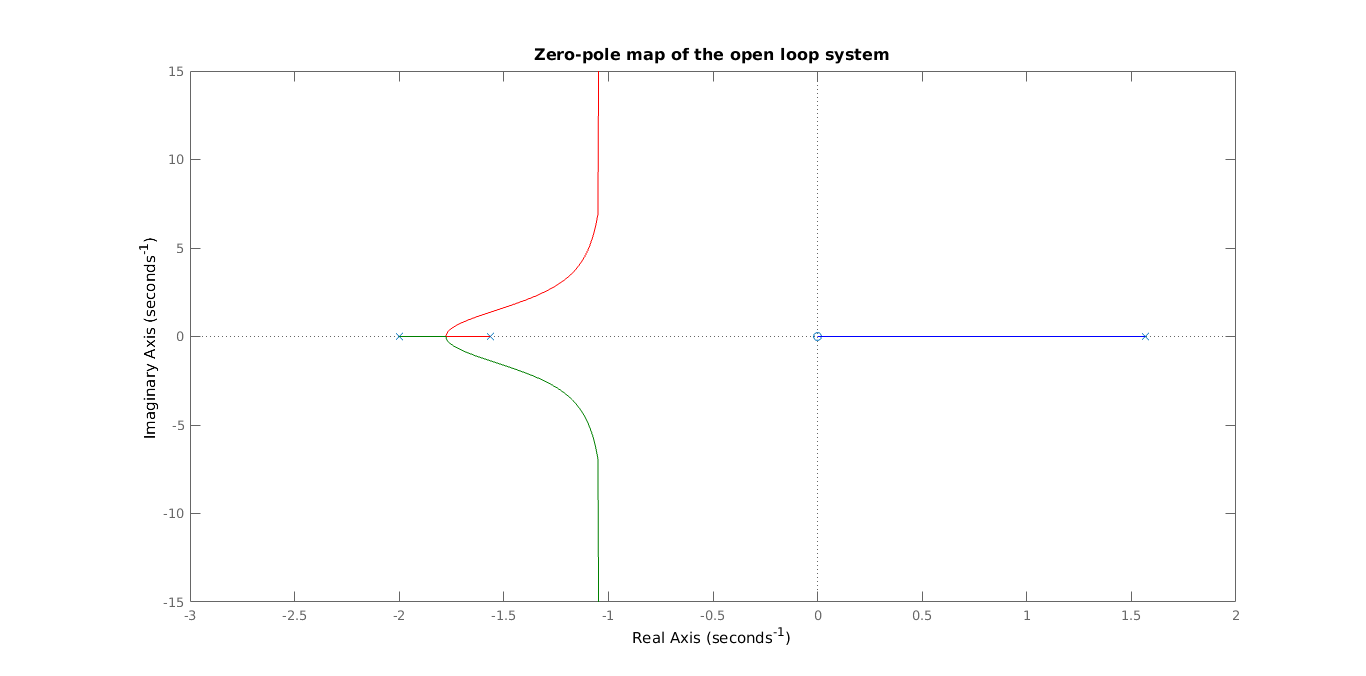
\includegraphics[scale=0.3]{rlocus-open-A.png}
	\caption{Zero-pole diagram for the open-loop system}\label{fig:zpopenA}
\end{figure}

The open-loop response shown in figure \ref{fig:openrespA} confirms the unstable behavior.

\begin{figure}[h]
	\centering
	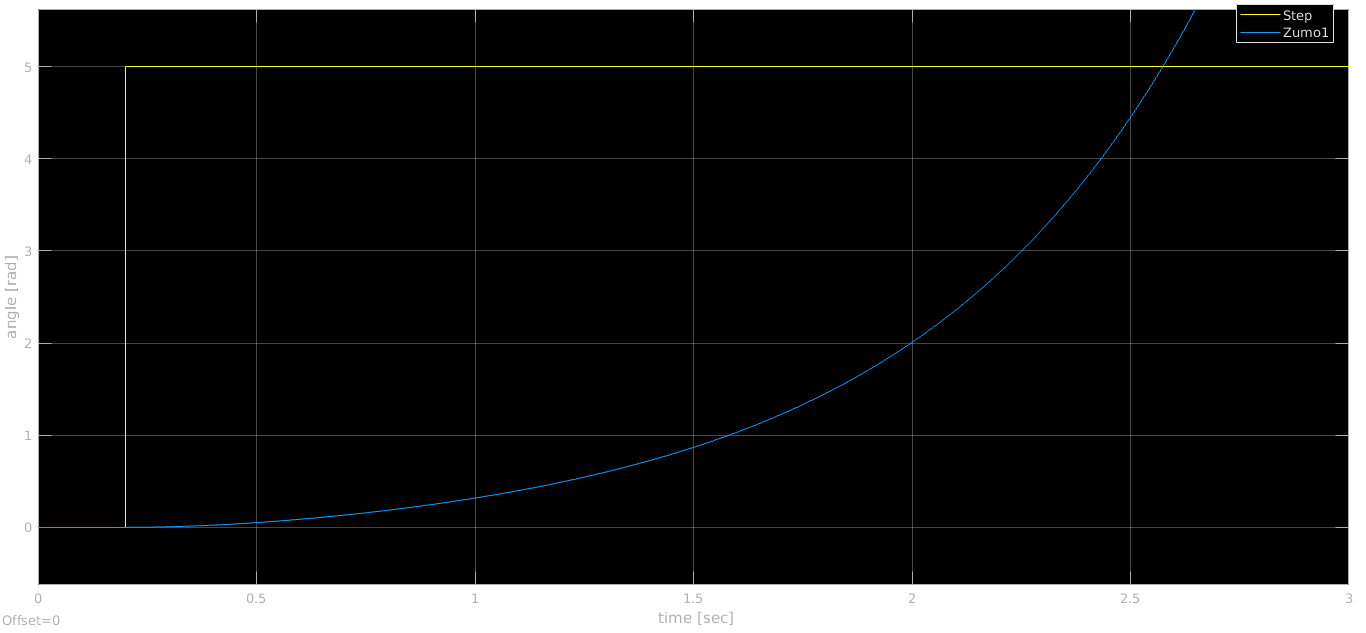
\includegraphics[scale=0.3]{open-loop-stepA.png}
	\caption{Open-loop step response of the system}\label{fig:openrespA}
\end{figure}

\section{Second approach - Euler-Lagrange}

\subsection{Dynamic behavior}

To represent the dynamics of the system as in \cite{JER12} and \cite{LUN02}, the initial definition is the natural form of the Lagrangian in classical mechanics:

\begin{equation} \label{nfl}
	\mathcal{L}=E_k-E_p
\end{equation}

Where $E_k=\frac{1}{2}mv^2$ and $E_p=mgh$. Equation \ref{nfl} can then be rewriten as:

\begin{equation} \label{nflr}
	\mathcal{L}=\frac{1}{2}mv^2-mgh
\end{equation}

The Euler-Lagrange equation states that:

\begin{equation} \label{ele}
	\frac{d}{dt}\left( \frac{\partial\mathcal{L}}{\partial\dot{\theta}} \right)=\frac{\partial\mathcal{L}}{\partial\theta}
\end{equation}

The pendulum is a stiff bar of lenght L which is supported at one end by a frictionless pin. From the figure \ref{fig:xypend} we can state that:

\begin{figure}[h]
	\centering
	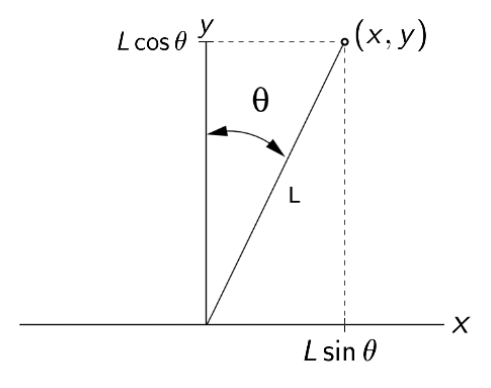
\includegraphics[scale=0.6]{xy-pendulum.png}
	\caption{Pendulum position}\label{fig:xypend}
\end{figure}

\begin{equation} \label{coord}
	\begin{aligned}
		x&=L\sin{\theta} & \dot{x}&=L\cos{\theta}\dot{\theta}\\
		y&=L\cos{\theta} & \dot{y}&=-L\sin{\theta}\dot{\theta}
	\end{aligned}
\end{equation}

Velocity is a vector representing the change in the position in the coordinates $x$ and $y$. Hence:

\begin{equation} \label{vel}
	v^2=\dot{x}^2+\dot{y}^2
\end{equation}

With the coordinates found in \ref{coord}, we can substitute in \ref{vel} to obtain:

\begin{equation} \label{vels}
	\begin{split}
		v^2&=L^2\cos{\theta}^2\dot{\theta}^2+L^2\sin{\theta}^2\dot{\theta}^2\\
		v^2&=L^2\dot{\theta}^2
	\end{split}
\end{equation}

Substituting \ref{coord} and \ref{vels} into \ref{nflr}, we obtain:

\begin{equation} \label{les}
	\mathcal{L}=\frac{1}{2}mL^2\dot{\theta}^2-mgL\cos{\theta}
\end{equation}

To perform the Euler-Lagrange equation presented in \ref{ele}, we need to compute the partial derivatives. First we compute the left part:

\begin{equation} \label{dlrt}
	\frac{\partial\mathcal{L}}{\partial\theta}=mgL\sin{\theta}
\end{equation}

Now we compute the inner part of the right element:

\begin{equation} \label{dlrtd}
	\frac{\partial\mathcal{L}}{\partial\dot{\theta}}=mL^2\dot{\theta}
\end{equation}

And now we can compute the outer derivative of \ref{dlrtd}:

\begin{equation} \label{dlrtt}
	\frac{d}{dt}\left( \frac{\partial\mathcal{L}}{\partial\dot{\theta}} \right)=mL^2\ddot{\theta}
\end{equation}

Now that we have all the terms, we can write the equation:

\begin{equation} \label{eles}
	\begin{split}
		\frac{d}{dt}\left( \frac{\partial\mathcal{L}}{\partial\dot{\theta}} \right)&=\frac{\partial\mathcal{L}}{\partial\theta}\\
		mL^2\ddot{\theta}&=mgL\sin{\theta}\\
		\ddot{\theta}&=\frac{g}{l}\sin{\theta}
	\end{split}
\end{equation}

Following the same procedure, we obtain the expression for the angular acceleration produced by the cart:

\begin{equation} \label{aac}
	\ddot{\theta}_x=\frac{\ddot{x}}{l}\cos{\theta}
\end{equation}

The total accelerations present on the pendulum can then be stated as:

\begin{equation} \label{saa}
	\ddot{\theta}=\ddot{\theta}_g+\ddot{\theta}_x=\left(\frac{g}{l}\right)\sin{\theta}-\left(\frac{\ddot{x}}{l}\right)\cos{\theta}
\end{equation}

The obtained equation is non-linear, so we apply an approximation based on the fact that the operation point implies an angle $\theta\approx0$. It means that $\sin{\theta}\approx\theta$ and $\cos{\theta}\approx1$. Applying this on \ref{saa}, we obtain:

\begin{equation} \label{lesa}
	l\ddot{\theta}-g\theta=-\ddot{x}
\end{equation}

To obtain the transfer function, we perform the Laplace transform on \ref{lesa}:

\begin{equation} \label{ltsa}
	ls^2\Theta(s)-g\Theta(s)=-s^2X(s)
\end{equation}

Now we solve for the variables $\Theta$ and $X$:

\begin{equation} \label{tfsa}
	\frac{\Theta(s)}{X(s)}=\frac{-s^2}{ls^2-g}
\end{equation}

\subsection{Actuator system}

For the motor modeling, a recommended approach \cite{LUN02} is used. The motor is diven by a voltage proportional to the angle:

\begin{equation} \label{mtf2}
	\frac{X(s)}{V(s)}=\frac{k_M}{s(\tau_M s+1)}
\end{equation}



\subsection{Simulation}

With the obtained model, a simulation in open-loop condition is run. As expected, the system contains a pole in the right part of the complex plane.

\begin{figure}[h]
	\centering
	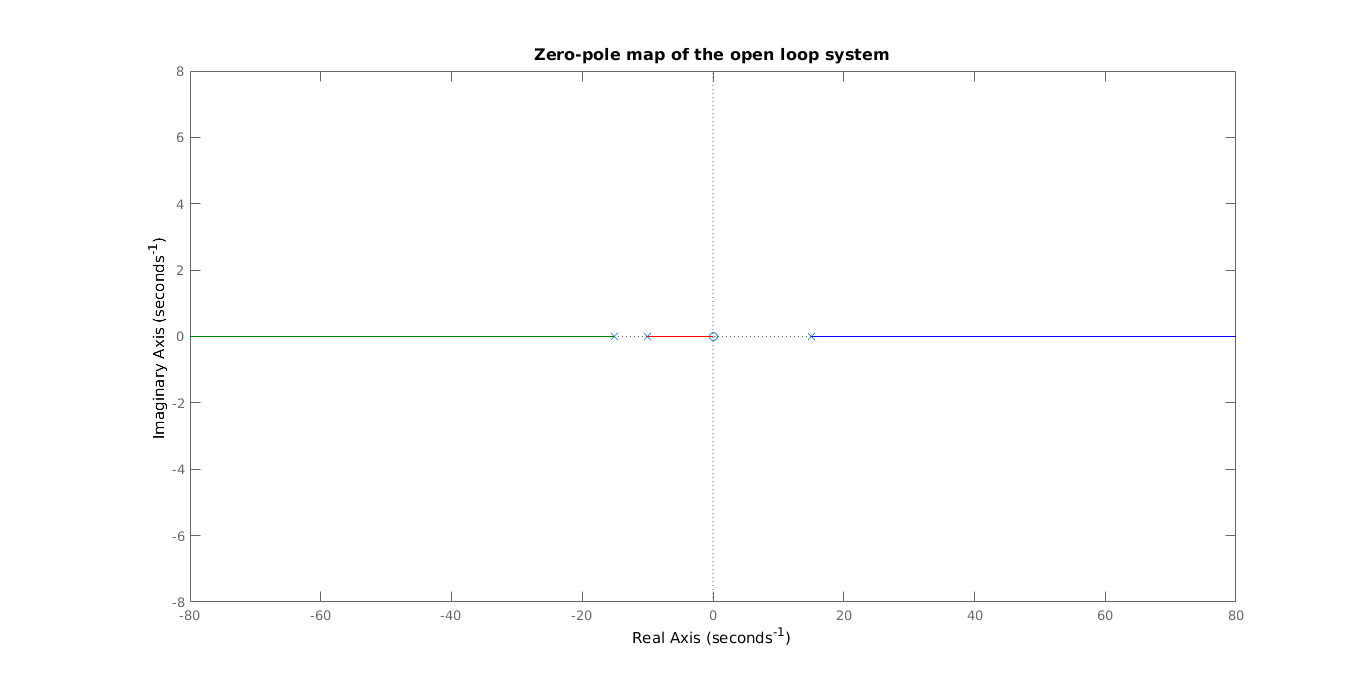
\includegraphics[scale=0.3]{rlocus-open-B.png}
	\caption{Zero-pole diagram for the open-loop system}\label{fig:zpB}
\end{figure}

The system response to a step input shows total unstability, as in figure \ref{fig:stepB}.

\begin{figure}[h]
	\centering
	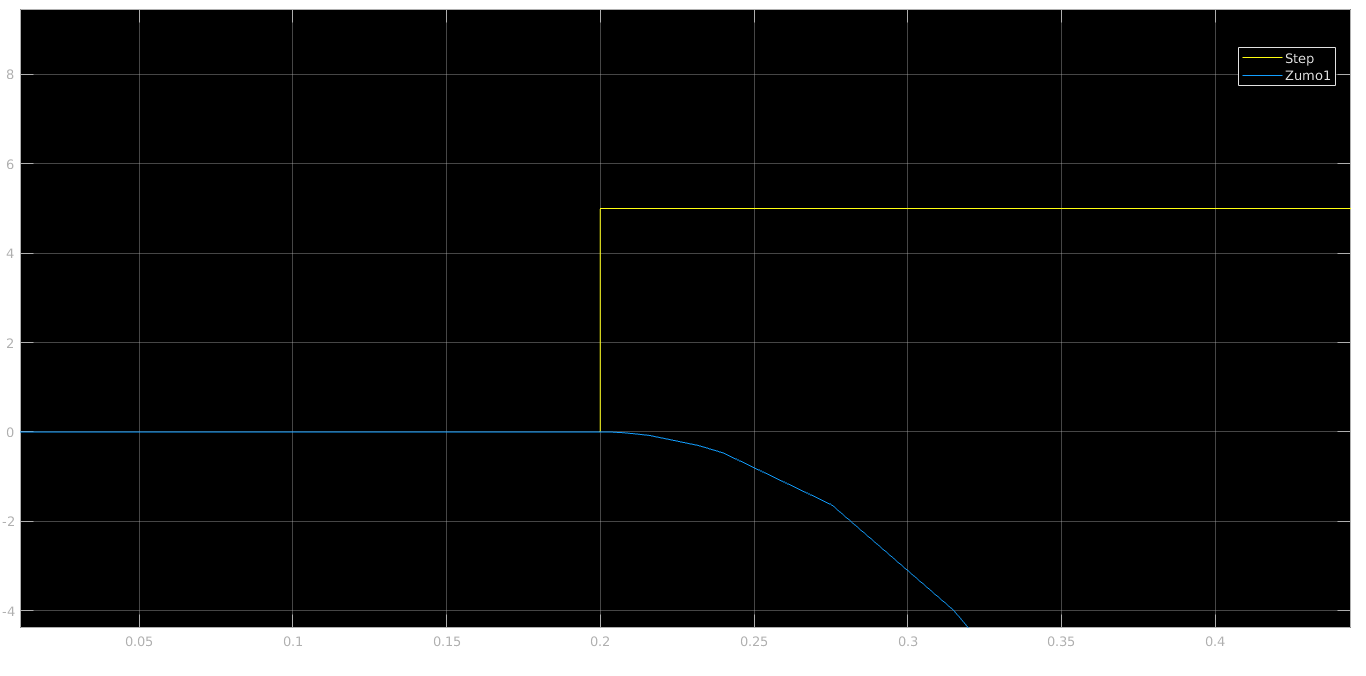
\includegraphics[scale=0.3]{open-loop-stepB.png}
	\caption{Open-loop step response of the system}\label{fig:stepB}
\end{figure}

This model is entirely more theoretical, and lacks of inclusion of physical parameters, so it is held as a second option.


% Inserts chapter from external file
\chapter{Control Design}
% Start of Chapter 3 - Control Design

From the obtained model, it is clear that the system needs a controller to govern the signal control, proportionally to the error (the pole on the right part needs to be canceled). For that reason, a PID parallel controller is the first step in the control work flow.

\section{Simulated controller}

With help of the computational tool (MATLAB), it is nowadays easy to tune a controller with desired specifications. The current version includes a GUI tool that allows to move around the different control specifications for the selected system, checking continuously the result. It certainly reduces time and effort in the calculations and design.

In this work, several different sets of constant definitions were made, with different simulated results. All of them

\section{Implemented controller}

The implemented controller was based on a common firmware provided by the Arduino community to be executed in the ATmega32U4 microcontroller. The source code is freely distributed to use and modify by the Zumo32U4 library repository. The algorithm executes the following steps:

\begin{enumerate}
	\item Calibration process of the accuracy of the measured values of the gyroscope, with help of the accelerometer.
	\item Main loop process:
	\begin{enumerate}
		\item Calculation of the current angle of the robot.
		\item Estimation of the weight of the measurement.
		\item Calculation of the difference between the desired and current angle.
		\item Calculation of PID control signal.
		\item Application of the control signal to the DC motor driver.
	\end{enumerate}
\end{enumerate}

\section{Results analysis}

The results of this work were not as satisfactory as expected, due to the bad behavior obtained from the Zumobot with the different designed controllers. It is clear that several reasons contribute to this factor, some of them can be stated as follows.

\subsection{Insufficient model}

The Zumobot has unique physical characteristics that cannot be represented with the model used. A bigger and complex system model needs to be defined that allows the representation of the real dimensions of the robot.

One of the biggest sources of disparity is the dynamic simulation of the free fall of the robot, due to the assumption of the mass, mass distribution, center of gravity and inertia. This values magnify the error in the expected response of the system, and consequently the controller is ineffective.

Another discrepancy in the model is the continuous-discrete difference. The digital implementation of the controller makes necessary to contemplate the plant as a discrete system, as all the measurements are taken in a fixed, discretized manner.

Finally, the management of the units in the modeling was careful in terms of units consistency, but there is a possibility that the small values for angle measurement in degrees cause errors in integer division operations on the Arduino architecture. A better approach with angle measured in radians can be used instead.

\subsection{Insufficient control technique}

The PID is one of the most basic control techniques for both stable and unstable systems. It simplicity and robustness equilibrium makes it a great choice for several applications.

Based on the learnings on this work, it might be a better choice to consider controller types less dependency of the accuracy of the error, and that offer better response in a wider range of operation. The linearized model used in this work shows a very small range where it can be valid.


\linespread{1.2}
\setlength{\parskip}{1em}

% Inserts the bibliography contained in report.bib, include no cited
\printbibliography%
\nocite{*}

\end{document}
